\section{Experiments on a laboratory shaker - Test 2}
In the previous section, the first test on the shaker was presented. The test shown the capability of the framework to detect unknown harmonics. A second test was done to evaluate the capability to detect time domain variations and the effect of reducing the frequency resolution. 

\subsection{Training and evaluating}
This new configuration has been set to use only 4 frequency-domain features and the same 3 time-domain features of the previous test, for a total of 7 features. The signal used for training and testing are resumed in \autoref{tab:shaker_param_02}. The set is composed by the same signal at different amplitudes used for training and testing, plus another signal with different frequency content but the same amplitude as a training signal used for testing. 

The training has been carried out in the same way of the previous test, the training of the K-means model has been done with 4 clusters, and loaded on the microcontroller. 

\begin{table}
    \centering
    \caption{Parameters of the second shaker test.}
    \label{tab:shaker_param_02}
    \begin{tabular}{cccccccc} 
    \toprule
    \multicolumn{5}{c}{\textbf{Harmonic frequency} {[}Hz]} & \multirow{2}{*}{\textbf{Amplitude }{[}mV$_{pp}$]} & \multicolumn{2}{c}{\textbf{ No. of snapshots}} \\
    10 & 30 & 60 & 70 & 100 &  & Train & Test \\ 
    \hline
    - & 0.1 & - & 1.0 & 1.0 & 580 & 100 & 10 \\
    - & 0.1 & - & 1.0 & 1.0 & 1000 & 100 & 10 \\
    - & 0.1 & - & 1.0 & 1.0 & 1980 & 100 & 10 \\
    - & 0.1 & - & 1.0 & 1.0 & 1540 & 100 & 10 \\
    - & 0.1 & - & 1.0 & 1.0 & 2000 & - & 20 \\
    - & 0.1 & - & 1.0 & 1.0 & 0 & - & 10 \\
    - & 0.1 & - & 1.0 & 1.0 & 800 & - & 10 \\
    - & 0.1 & - & 1.0 & 1.0 & 200 & - & 10 \\
    - & 0.1 & - & 1.0 & 1.0 & 1220 & - & 10 \\
    1.0 & 1.0 & 0.1 & - & - & 1540 & - & 10 \\
    \bottomrule
    \end{tabular}
    \end{table}



\subsection{Results}
\begin{figure}
    \centering
    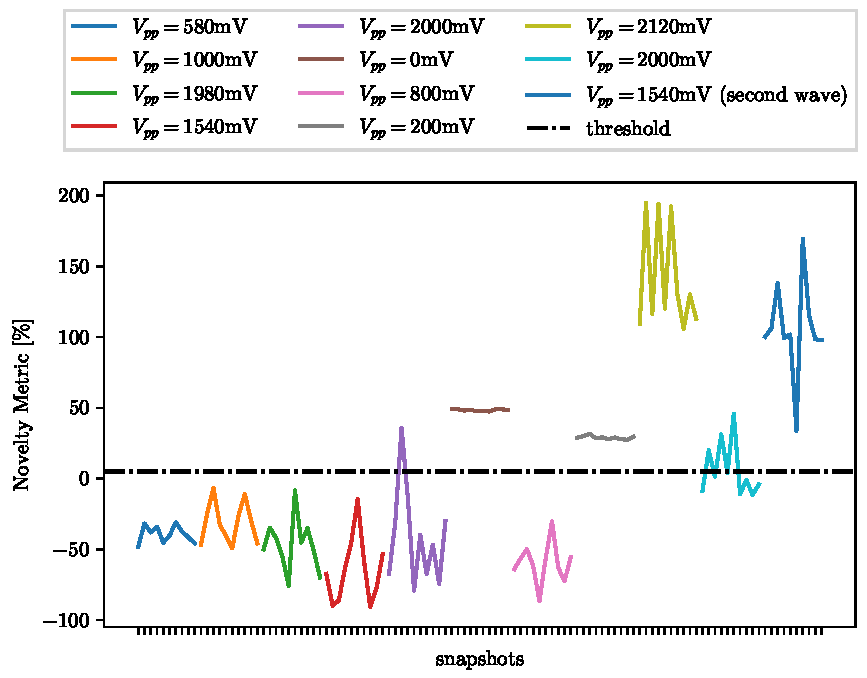
\includegraphics{Images/shaker/Test02.pdf}
    \caption{Novelty detection result}
    \label{fig:shaker_results02}
\end{figure}
The result of the novelty detection is shown in \autoref{fig:shaker_results02}. The first 4 lines has been correctly identified as normal, as they was in fact a repetition of the training signals.
Then the purple and cyan line in the figure is the same training signal, but 20 mV higher in amplitude \gls{wrt} the training signal. The novelty metric overshoots the threshold in 5 samples out of 20. An increase of 2\% in amplitude generates the \gls{nd} event 25\% of the times can be observed with this signal. 

The brown, grey and light-green lines are the same signal, but with a bigger difference in amplitude \gls{wrt} the training signal. All the snapshots of theese signals correctly generated a novelty metric above the treshold. The blue line is the signal with a different frequency content, and it has been correctly identified as a novelty event, this is the confirmation that even with just 4 frequency bins, the wavelet decomposition is still generating features that are informative.

The pink line is the test signal with anplitude of 800mV. It's evident that the novelty metric is below the threshold, and the signal has been classified as normal even if it is not in the trai dataset. Let's investigate how this happened. The first consideration is that the 800mV amplitude is quite tight to both the 1000mv and 580mV signals used for training. Moreover, in this case, the total number of features is just 7. This allows to plot all the features against each other, to see why the \gls{nd} event has not been detected. In \autoref{fig:shaker_conf_matrix} the scatter plot of the features is shown. It's evident that , in this envinronment, even performing the standardization of the features, the clusters are still very elongated, resempling almost a line. To fit an elongated cluster in a hypersphere, it is inevitable that in some section, the hypersphere will not closely sorround the cluster, leaving \quoted{space} for false negative results. Another problem is that the k-means algorithm would tend to split long clusters. In the figure, the red dots are the false negative results, and the gray shades are the hypersphere projection on the sonsidered features plane. The black dots are the training data. The effect of the elongated clusters is particularly evident in the plot of the \quoted{Feature 3} against \quoted{Feature 2}, where the red dots are in between two clusters, that are modelled as one. On the other hand, looking at the plot of \quoted{Feature 1} against \quoted{Feature 4}, a very long cluster has been split in two. This is an example of exploiting the limitations of the k-means algorithm anticipated in \autoref{sec:kmeans_limits}. 
For completness, in \autoref{fig:shaker_conf_matrix}, also the true positive results are shown, as magenta dots.


\begin{figure}
    \centering
    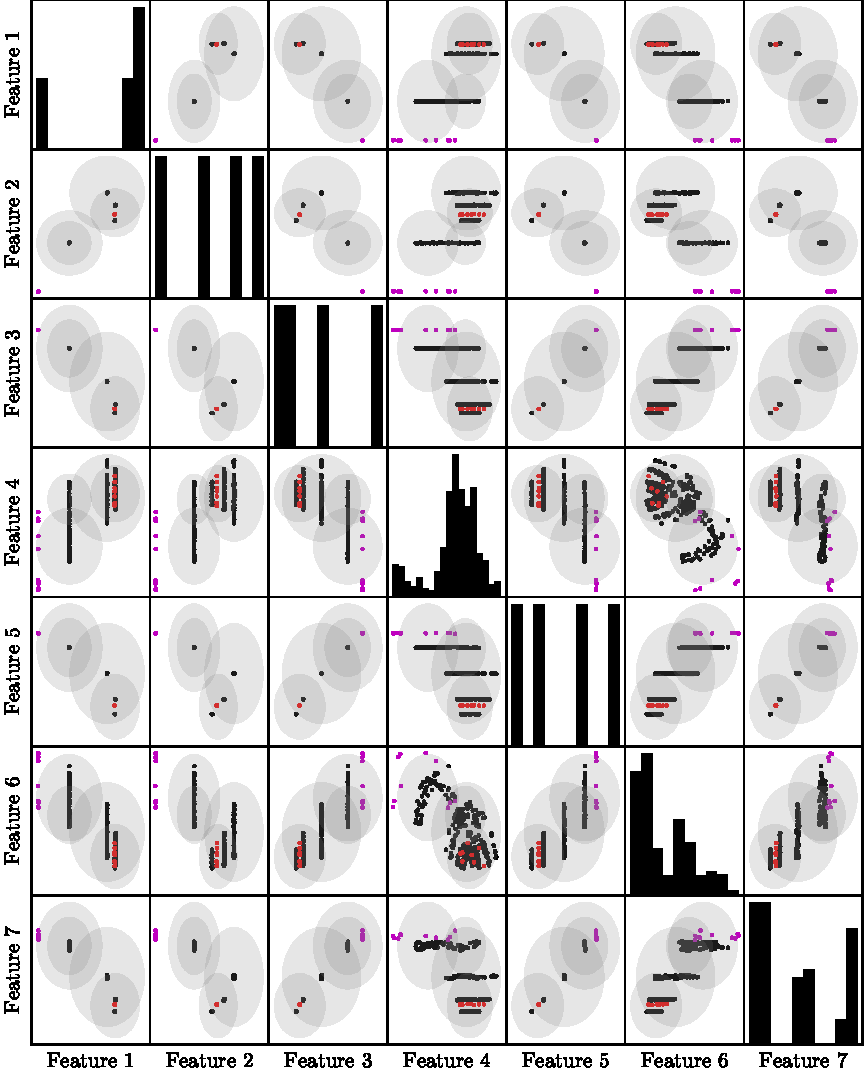
\includegraphics{Images/shaker/ConfusionMatrix.pdf}
    \caption{False Negative and True Positive results. On the diagonal, there is an histogram of the feature values. The off-diagonal plots are the scatter plots of the features. The shades are the projection of the clusters on the considered plane. (Red: False Negative, Magenta: True Positive, Black: training data)}
    \label{fig:shaker_conf_matrix}
\end{figure}

\subsection{Possible improvements}
The envinronment of this test is very challenging for the k-means algorithm. As discussed in \autoref{ch:Unsupervised}, there are algorithms that are not affected by the clusters shapes. The candidates algorithms that may perform better in this situation are the \gls{lof}, the \gls{iforest} and \gls{dbscan}. A futue work could be to implement these algorithms in the \gls{glo:edge} framework, despite being them more demanding in camputational power and memory, and test them in this environment.

As proof of concept, the \gls{lof} implementation in \texttt{python} has been used to perform \gls{nd} on the same dataset used in this section in \gls{glo:edge}. The results are reported in \autoref{label:lof_results}. The \gls{lof} algorithm has been able to correctly identify all the \gls{nd} events, even the signals with just 20mV variation from the training dataset, and the 800mV signal that was problematic fot the K-means. The \gls{lof}, however, generated a false positive on the 580mV signal. This false positice may be avoided by increasing the threshold, but this would also increase the false negative rate. 

\begin{figure}
    \centering
    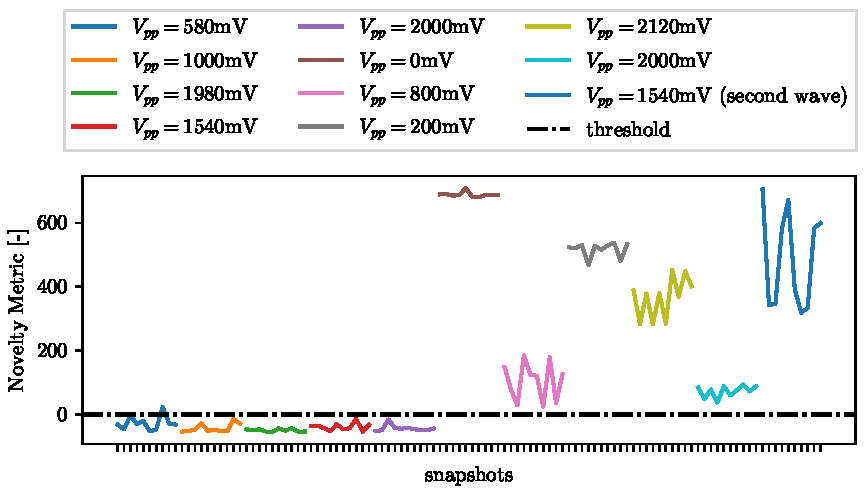
\includegraphics{Images/shaker/Test02_LOF.pdf}
    \caption{\gls{lof} novelty detection result}
    \label{fig:lof_results}
\end{figure}